% Options for packages loaded elsewhere
\PassOptionsToPackage{unicode}{hyperref}
\PassOptionsToPackage{hyphens}{url}
%
\documentclass[
  ignorenonframetext,
]{beamer}
\usepackage{pgfpages}
\setbeamertemplate{caption}[numbered]
\setbeamertemplate{caption label separator}{: }
\setbeamercolor{caption name}{fg=normal text.fg}
\beamertemplatenavigationsymbolsempty
% Prevent slide breaks in the middle of a paragraph
\widowpenalties 1 10000
\raggedbottom
\setbeamertemplate{part page}{
  \centering
  \begin{beamercolorbox}[sep=16pt,center]{part title}
    \usebeamerfont{part title}\insertpart\par
  \end{beamercolorbox}
}
\setbeamertemplate{section page}{
  \centering
  \begin{beamercolorbox}[sep=12pt,center]{part title}
    \usebeamerfont{section title}\insertsection\par
  \end{beamercolorbox}
}
\setbeamertemplate{subsection page}{
  \centering
  \begin{beamercolorbox}[sep=8pt,center]{part title}
    \usebeamerfont{subsection title}\insertsubsection\par
  \end{beamercolorbox}
}
\AtBeginPart{
  \frame{\partpage}
}
\AtBeginSection{
  \ifbibliography
  \else
    \frame{\sectionpage}
  \fi
}
\AtBeginSubsection{
  \frame{\subsectionpage}
}
\usepackage{amsmath,amssymb}
\usepackage{lmodern}
\usepackage{ifxetex,ifluatex}
\ifnum 0\ifxetex 1\fi\ifluatex 1\fi=0 % if pdftex
  \usepackage[T1]{fontenc}
  \usepackage[utf8]{inputenc}
  \usepackage{textcomp} % provide euro and other symbols
\else % if luatex or xetex
  \usepackage{unicode-math}
  \defaultfontfeatures{Scale=MatchLowercase}
  \defaultfontfeatures[\rmfamily]{Ligatures=TeX,Scale=1}
\fi
\usetheme[]{Boadilla}
% Use upquote if available, for straight quotes in verbatim environments
\IfFileExists{upquote.sty}{\usepackage{upquote}}{}
\IfFileExists{microtype.sty}{% use microtype if available
  \usepackage[]{microtype}
  \UseMicrotypeSet[protrusion]{basicmath} % disable protrusion for tt fonts
}{}
\makeatletter
\@ifundefined{KOMAClassName}{% if non-KOMA class
  \IfFileExists{parskip.sty}{%
    \usepackage{parskip}
  }{% else
    \setlength{\parindent}{0pt}
    \setlength{\parskip}{6pt plus 2pt minus 1pt}}
}{% if KOMA class
  \KOMAoptions{parskip=half}}
\makeatother
\usepackage{xcolor}
\IfFileExists{xurl.sty}{\usepackage{xurl}}{} % add URL line breaks if available
\IfFileExists{bookmark.sty}{\usepackage{bookmark}}{\usepackage{hyperref}}
\hypersetup{
  pdftitle={Environmental Legislation and its Effects on Air Quality},
  pdfauthor={Group 2},
  hidelinks,
  pdfcreator={LaTeX via pandoc}}
\urlstyle{same} % disable monospaced font for URLs
\newif\ifbibliography
\usepackage{graphicx}
\makeatletter
\def\maxwidth{\ifdim\Gin@nat@width>\linewidth\linewidth\else\Gin@nat@width\fi}
\def\maxheight{\ifdim\Gin@nat@height>\textheight\textheight\else\Gin@nat@height\fi}
\makeatother
% Scale images if necessary, so that they will not overflow the page
% margins by default, and it is still possible to overwrite the defaults
% using explicit options in \includegraphics[width, height, ...]{}
\setkeys{Gin}{width=\maxwidth,height=\maxheight,keepaspectratio}
% Set default figure placement to htbp
\makeatletter
\def\fps@figure{htbp}
\makeatother
\setlength{\emergencystretch}{3em} % prevent overfull lines
\providecommand{\tightlist}{%
  \setlength{\itemsep}{0pt}\setlength{\parskip}{0pt}}
\setcounter{secnumdepth}{-\maxdimen} % remove section numbering
\AtBeginSection[]{\begin{frame}\tableofcontents[currentsection]\end{frame}}
\AtBeginSubsection[]{\begin{frame}\tableofcontents[currentsubsection]\end{frame}{}}
\ifluatex
  \usepackage{selnolig}  % disable illegal ligatures
\fi

\title{Environmental Legislation and its Effects on Air Quality}
\author{Group 2}
\date{}

\begin{document}
\frame{\titlepage}

\hypertarget{introduction}{%
\subsection{Introduction}\label{introduction}}

\begin{frame}{Introduction}
The goal of this study is to examine the impact of certain variables on
the climate by examining the AQI of counties across the United States of
America using data collected by the EPA.

There are two smaller sub studies in this presentation: One examining
the effects of the Climate Alliance legislative program, and another
examining the correlation between aspects of counties and the air
quality.
\end{frame}

\hypertarget{reading-the-data-and-eda}{%
\subsection{Reading the Data and EDA}\label{reading-the-data-and-eda}}

\begin{frame}[fragile]
\frametitle{Read and Clean}

To begin we read the data in from the EPA datasets.

\tiny

\begin{verbatim}
## `summarise()` has grouped output by 'state'. You can override using the `.groups` argument.
\end{verbatim}
\end{frame}

\begin{frame}
\frametitle{Heatmap}

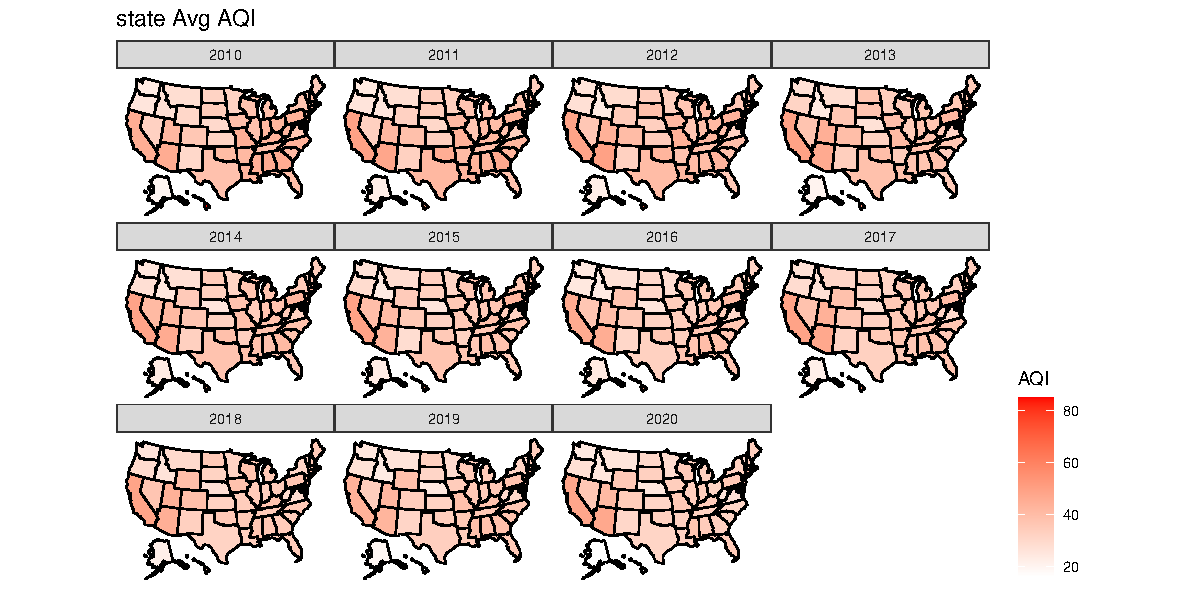
\includegraphics{final_files/figure-beamer/heatmap-1.pdf}
\end{frame}

\begin{frame}
\frametitle{AQI by Year Faceted by State}

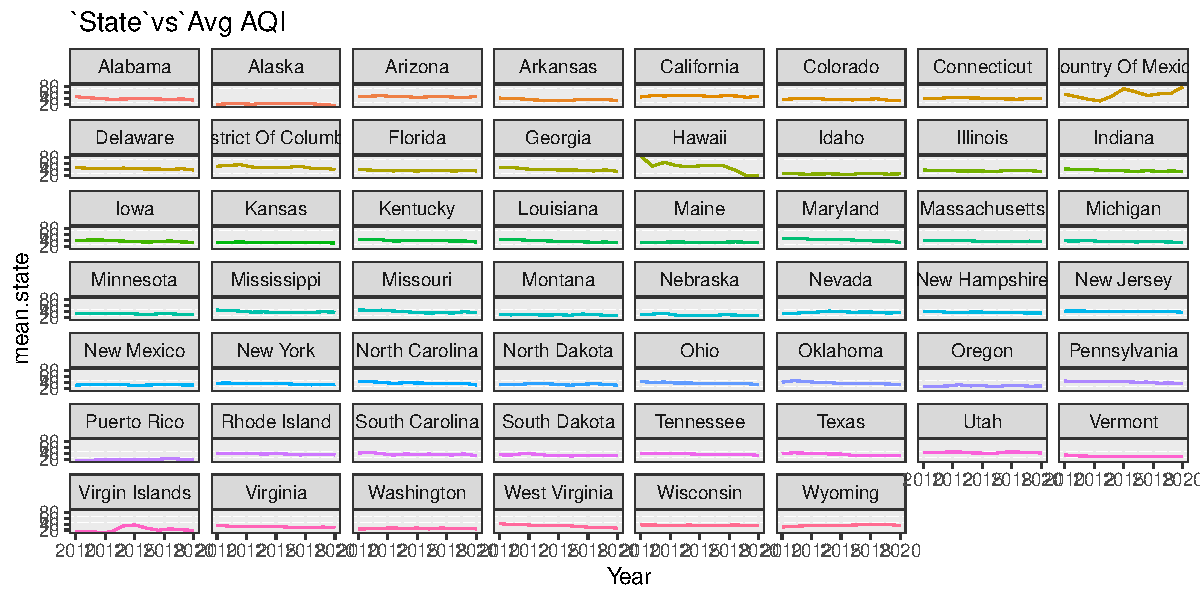
\includegraphics{final_files/figure-beamer/facetAqi-1.pdf}
\end{frame}

\hypertarget{climate-alliance}{%
\subsection{Climate Alliance}\label{climate-alliance}}

\begin{frame}[fragile]
\frametitle{Linear Regression}

\begin{verbatim}
## 
## Call:
## lm(formula = med.aqi ~ is.climate.alli + state, data = focus_data)
## 
## Residuals:
##    Min     1Q Median     3Q    Max 
## -36.82  -3.06   1.36   5.68  94.52 
## 
## Coefficients: (1 not defined because of singularities)
##                           Estimate Std. Error t value Pr(>|t|)    
## (Intercept)                37.5294     1.8246   20.57  < 2e-16 ***
## is.climate.alliyes         -1.1008     2.3131   -0.48  0.63418    
## stateAlaska               -17.0000     3.1602   -5.38  8.3e-08 ***
## stateArizona                6.3167     2.7717    2.28  0.02277 *  
## stateArkansas              -1.7294     2.8029   -0.62  0.53730    
## stateCalifornia             9.8827     1.7575    5.62  2.1e-08 ***
## stateColorado               0.3419     1.9689    0.17  0.86215    
## stateConnecticut            2.1339     3.0158    0.71  0.47929    
## stateCountry Of Mexico     18.9706     5.6237    3.37  0.00076 ***
## stateDelaware               4.7381     4.5701    1.04  0.29997    
## stateDistrict Of Columbia   6.4706     7.7409    0.84  0.40331    
## stateFlorida               -2.3371     2.1864   -1.07  0.28522    
## stateGeorgia               -0.8570     2.2979   -0.37  0.70923    
## stateHawaii                -8.4286     4.0211   -2.10  0.03620 *  
## stateIdaho                -12.5294     2.4544   -5.10  3.6e-07 ***
## stateIllinois              -1.1323     2.0291   -0.56  0.57689    
## stateIndiana               -3.4669     2.1780   -1.59  0.11159    
## stateIowa                  -1.2169     2.6203   -0.46  0.64240    
## stateKansas                -5.2112     2.9110   -1.79  0.07357 .  
## stateKentucky               0.5261     2.3292    0.23  0.82131    
## stateLouisiana             -2.4068     2.1170   -1.14  0.25571    
## stateMaine                 -2.0786     2.7714   -0.75  0.45333    
## stateMaryland               1.3950     2.3131    0.60  0.54652    
## stateMassachusetts         -0.2986     2.7717   -0.11  0.91421    
## stateMichigan              -1.5536     2.0106   -0.77  0.43979    
## stateMinnesota             -5.7857     2.1717   -2.66  0.00778 ** 
## stateMississippi           -0.0056     2.9528    0.00  0.99849    
## stateMissouri              -1.0502     2.3847   -0.44  0.65969    
## stateMontana               -9.6610     2.5115   -3.85  0.00012 ***
## stateNebraska             -11.4739     3.1012   -3.70  0.00022 ***
## stateNevada                -0.9286     2.8826   -0.32  0.74739    
## stateNew Hampshire         -2.8151     3.3784   -0.83  0.40479    
## stateNew Jersey             2.5089     2.3576    1.06  0.28737    
## stateNew Mexico            -4.2411     2.3576   -1.80  0.07218 .  
## stateNew York              -4.9608     1.9613   -2.53  0.01150 *  
## stateNorth Carolina        -0.4549     1.8736   -0.24  0.80820    
## stateNorth Dakota          -3.2794     2.9981   -1.09  0.27415    
## stateOhio                  -2.4104     2.1625   -1.11  0.26515    
## stateOklahoma              -2.5702     2.3746   -1.08  0.27922    
## stateOregon                -8.5350     2.1046   -4.06  5.2e-05 ***
## statePennsylvania           0.9294     1.8489    0.50  0.61523    
## statePuerto Rico          -15.4841     2.8826   -5.37  8.7e-08 ***
## stateRhode Island          -0.4286     4.5701   -0.09  0.92529    
## stateSouth Carolina        -1.5016     2.5442   -0.59  0.55511    
## stateSouth Dakota          -5.8794     2.9981   -1.96  0.05000 .  
## stateTennessee             -1.9425     2.4061   -0.81  0.41959    
## stateTexas                 -4.8593     2.1204   -2.29  0.02202 *  
## stateUtah                   5.7039     2.6649    2.14  0.03244 *  
## stateVermont               -7.0536     4.0211   -1.75  0.07956 .  
## stateVirgin Islands       -14.8628     4.7110   -3.15  0.00163 ** 
## stateVirginia              -6.9139     1.9198   -3.60  0.00032 ***
## stateWashington           -10.7892     1.9689   -5.48  4.8e-08 ***
## stateWest Virginia         -8.3732     2.6203   -3.20  0.00142 ** 
## stateWisconsin                  NA         NA      NA       NA    
## stateWyoming                1.6650     2.5442    0.65  0.51290    
## ---
## Signif. codes:  0 '***' 0.001 '**' 0.01 '*' 0.05 '.' 0.1 ' ' 1
## 
## Residual standard error: 10.6 on 2055 degrees of freedom
## Multiple R-squared:  0.187,  Adjusted R-squared:  0.166 
## F-statistic: 8.92 on 53 and 2055 DF,  p-value: <2e-16
\end{verbatim}
\end{frame}

\begin{frame}
\frametitle{Analysis}

Climate Alliance states tend to have a better AQI on average but it is
not significant.

This might be because the Climate Alliance only went into effect 3 years
ago in 2017.
\end{frame}

\hypertarget{county-level-effects-on-aqi}{%
\subsection{County Level Effects on
AQI}\label{county-level-effects-on-aqi}}

\begin{frame}{County Level Effects on AQI}
Using the data found by the USDA's Economic Research Service, we look
for predictors in counties to determine air quality and find
correlations.

This begins by merging the 2019 AQI with the latest USDA ERS data. We
use 2019 data to avoid skewing due to the 2020 West Coast fires.
\end{frame}

\begin{frame}
\frametitle{Merging AQI Data with County Data}

To begin the analysis, we start by merging county data with AQI data. We
start by merging all three sets of ERS county data, and then we merge by
county and state.

We only take the data from year 2019 to keep it consistent. We are
avoiding using 2020 data due to the fires on the West coast skewing
data.

\tiny
\end{frame}

\begin{frame}[fragile]
\frametitle{Running the LASSO Algorithm}

Break the cleaned and merged dataset into X and Y for use with
cv.glmnet. We use set.seed(1) for consistency.

\tiny

\begin{verbatim}
## Note: Using an external vector in selections is ambiguous.
## i Use `all_of(select_cols)` instead of `select_cols` to silence this message.
## i See <https://tidyselect.r-lib.org/reference/faq-external-vector.html>.
## This message is displayed once per session.
\end{verbatim}

\begin{verbatim}
## Anova Table (Type II tests)
## 
## Response: med.aqi
##                      Sum Sq  Df F value  Pr(>F)    
## state                 15670  48    3.44 2.5e-13 ***
## PctEmpAgriculture       109   1    1.15  0.2848    
## PctEmpConstruction      174   1    1.83  0.1761    
## PctEmpFIRE              734   1    7.73  0.0055 ** 
## Age65AndOlderPct2010     50   1    0.53  0.4676    
## Ed4AssocDegreePct       774   1    8.16  0.0044 ** 
## FemaleHHPct            1681   1   17.71 2.8e-05 ***
## HH65PlusAlonePct        578   1    6.09  0.0138 *  
## Ed3SomeCollegeNum       737   1    7.77  0.0054 ** 
## ForeignBornMexNum       610   1    6.43  0.0114 *  
## NetMigrationNum0010    1698   1   17.90 2.6e-05 ***
## Residuals             89962 948                    
## ---
## Signif. codes:  0 '***' 0.001 '**' 0.01 '*' 0.05 '.' 0.1 ' ' 1
\end{verbatim}
\end{frame}

\begin{frame}[fragile]
\frametitle{Backwards Selection with Anova}

From the Anova call above, we see that Age65AndOlderPct2010 is the least
relevant, so we remove it.

\tiny

\begin{verbatim}
## Anova Table (Type II tests)
## 
## Response: med.aqi
##                     Sum Sq  Df F value  Pr(>F)    
## state                15623  48    3.43 2.9e-13 ***
## PctEmpAgriculture       92   1    0.97  0.3246    
## PctEmpConstruction     143   1    1.50  0.2205    
## PctEmpFIRE             723   1    7.62  0.0059 ** 
## Ed4AssocDegreePct      744   1    7.84  0.0052 ** 
## FemaleHHPct           1652   1   17.41 3.3e-05 ***
## HH65PlusAlonePct       950   1   10.01  0.0016 ** 
## Ed3SomeCollegeNum      732   1    7.72  0.0056 ** 
## ForeignBornMexNum      618   1    6.52  0.0108 *  
## NetMigrationNum0010   1683   1   17.74 2.8e-05 ***
## Residuals            90012 949                    
## ---
## Signif. codes:  0 '***' 0.001 '**' 0.01 '*' 0.05 '.' 0.1 ' ' 1
\end{verbatim}
\end{frame}

\begin{frame}[fragile]
\frametitle{Backwards Selection with Anova}

From the Anova call above, we see that PctEmpAgriculture is the least
relevant, so we remove it.

\tiny

\begin{verbatim}
## Anova Table (Type II tests)
## 
## Response: med.aqi
##                     Sum Sq  Df F value  Pr(>F)    
## state                16002  48    3.51 8.3e-14 ***
## PctEmpConstruction     124   1    1.31 0.25270    
## PctEmpFIRE            1037   1   10.93 0.00098 ***
## Ed4AssocDegreePct      685   1    7.22 0.00732 ** 
## FemaleHHPct           1667   1   17.58 3.0e-05 ***
## HH65PlusAlonePct      1046   1   11.03 0.00093 ***
## Ed3SomeCollegeNum      786   1    8.29 0.00408 ** 
## ForeignBornMexNum      614   1    6.47 0.01112 *  
## NetMigrationNum0010   1704   1   17.96 2.5e-05 ***
## Residuals            90104 950                    
## ---
## Signif. codes:  0 '***' 0.001 '**' 0.01 '*' 0.05 '.' 0.1 ' ' 1
\end{verbatim}
\end{frame}

\begin{frame}[fragile]
\frametitle{Backwards Selection with Anova}

From the Anova call above, we see that PctEmpConstruction is the least
relevant, so we remove it.

\tiny

\begin{verbatim}
## Anova Table (Type II tests)
## 
## Response: med.aqi
##                     Sum Sq  Df F value  Pr(>F)    
## state                16606  48    3.65 1.1e-14 ***
## PctEmpFIRE            1127   1   11.88 0.00059 ***
## Ed4AssocDegreePct      733   1    7.73 0.00555 ** 
## FemaleHHPct           1974   1   20.81 5.7e-06 ***
## HH65PlusAlonePct      1139   1   12.01 0.00055 ***
## Ed3SomeCollegeNum      814   1    8.58 0.00348 ** 
## ForeignBornMexNum      582   1    6.13 0.01347 *  
## NetMigrationNum0010   1679   1   17.69 2.8e-05 ***
## Residuals            90228 951                    
## ---
## Signif. codes:  0 '***' 0.001 '**' 0.01 '*' 0.05 '.' 0.1 ' ' 1
\end{verbatim}
\end{frame}

\begin{frame}[fragile]
\frametitle{Examining the Final Fit - Do the Assumptions of the Linear Model Hold Up?}

\tiny

\begin{verbatim}
##                      Estimate Std. Error t value Pr(>|t|)
## PctEmpFIRE           6.13e-01   1.78e-01    3.45 5.91e-04
## Ed4AssocDegreePct   -5.29e-01   1.90e-01   -2.78 5.55e-03
## FemaleHHPct          5.35e-01   1.17e-01    4.56 5.73e-06
## HH65PlusAlonePct    -4.73e-01   1.36e-01   -3.47 5.53e-04
## Ed3SomeCollegeNum    1.42e-05   4.86e-06    2.93 3.48e-03
## ForeignBornMexNum    2.15e-05   8.67e-06    2.48 1.35e-02
## NetMigrationNum0010  2.78e-05   6.61e-06    4.21 2.84e-05
\end{verbatim}

From the final model, we see that most of the impact on AQI is
geographical. For example, the increase from ForeignBornMexNum and
NetMigrationNum could signal that states closer to the Mexican border
tend to have worse AQIs due to their location. However, the most clear
predictors are the states themselves.

The assumptions for linearity appear to hold up until about 1 standard
deviation below the mean.
\end{frame}

\begin{frame}
\frametitle{Diagnostic Plots}

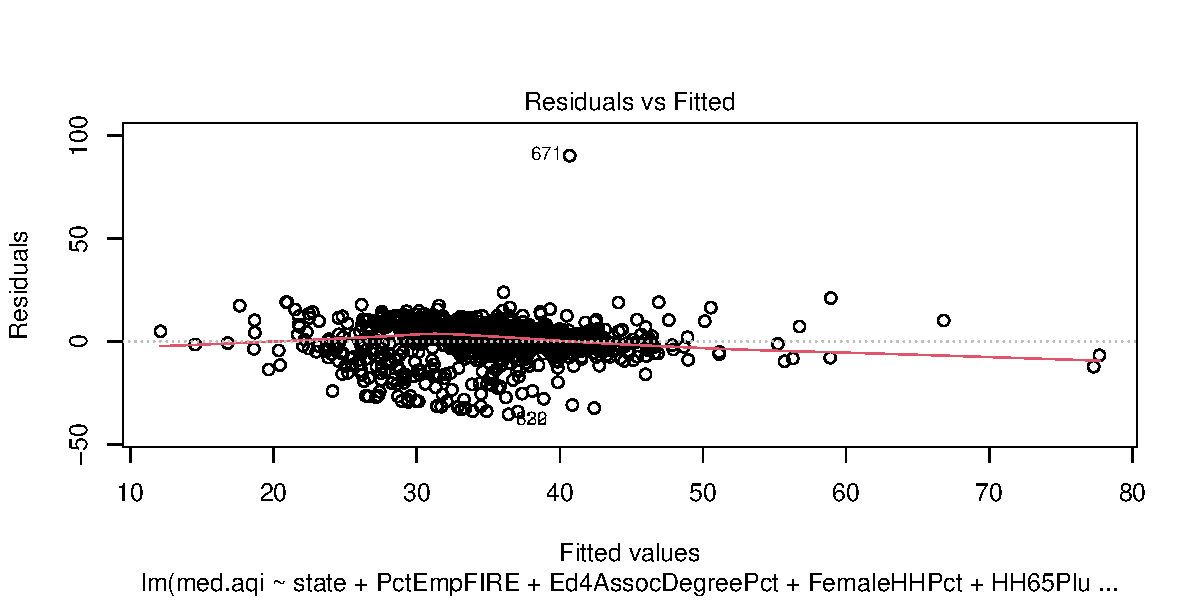
\includegraphics[width=0.5\linewidth]{final_files/figure-beamer/plots-1}
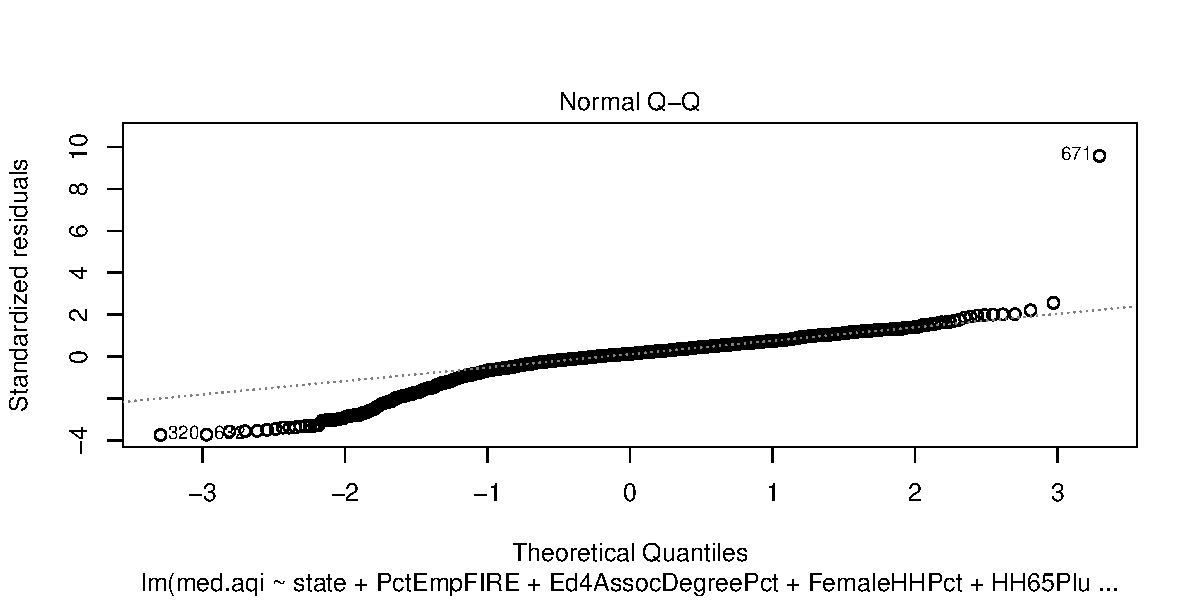
\includegraphics[width=0.5\linewidth]{final_files/figure-beamer/plots-2}
\#\# Conclusion

The overall objective of this study was to use the AQI of counties
across the USA to determine the impact of variables on the climate.
Using data collected by the EPA, we were able to focus on the effect of
the Climate Alliance on curbing the deterioration of the AQI across the
nation, as well as the correlation between aspects of counties and their
air quality.

From this study, we were able to conclude that the Climate Alliance has
not had much of an effect yet on the AQI of member states, but do have
better AQIs on average compared to other states. We were also able to
see that most of the impact on the AQI is geographical based on the
significant variables of the model.
\end{frame}

\end{document}
